\documentclass[11pt]{article}
\usepackage[margin=1in]{geometry}
\usepackage{graphicx}
\usepackage{booktabs}
\usepackage{float}
\usepackage{hyperref}
\usepackage{array}
\usepackage{caption}
\usepackage{longtable}
\usepackage{parskip}
\usepackage[T1]{fontenc}
\usepackage{lmodern}

\graphicspath{{../Data/}}
\hypersetup{
    colorlinks=true,
    linkcolor=black,
    urlcolor=blue,
    citecolor=black
}

\title{Can Nuclear Fusion Power a Mars Colony?\\INDENG 290 Final Project Report}
\author{Vineet Reddy \and Samuel Heinz \and Nicholas Fitzpatrick}
\date{Spring 2026}

\begin{document}

\maketitle

\begin{abstract}
This project compares solar, fission, and several fusion concepts for a Mars colony power system. We study the problem from three angles: feasibility, cost, and reliability under dust storms. The main result is consistent across the different analyses. Solar by itself is not reliable enough for the colony sizes we tested, fission performs well as the practical near term option, and fusion becomes interesting mainly as a long run scale argument rather than a near term engineering choice. The project repository, report source, and slide deck are available at \href{https://github.com/sjheinz17/MarsColonyNuclearFusion}{github.com/sjheinz17/MarsColonyNuclearFusion}.
\end{abstract}

\section{Introduction}

Future Mars missions will need continuous electric power for life support, thermal control, oxygen production, water recycling, communications, and general habitat operations. That requirement becomes harder on Mars because solar input is weaker than on Earth, nights are long, and dust storms can sharply reduce available solar power. The project was built around three questions:

\begin{enumerate}
    \item At what point does fusion start to look better than adding more fission units.
    \item How strongly do dust storms affect power reliability.
    \item Which fusion concept looks most credible on paper.
\end{enumerate}

The final scope is narrower than the original proposal in one important way. Fusion is not placed inside the sol by sol reliability simulator (one Martian day at a time) because we did not have a defensible way to model operational availability for systems that do not yet exist. Instead, fusion is evaluated through resource classification and cost modeling, while the reliability work focuses on solar and fission.

\section{Input Data and Provenance}

The project uses six input CSV files. Two are downloaded datasets and four are tables prepared by the team for the model. Most of the other CSV files in the \path{Data/} folder are generated outputs written by the code.

\begin{table}[H]
    \centering
    \small
    \caption{Input CSV files and where they came from.}
    \begin{tabular}{>{\raggedright\arraybackslash}p{1.55in}>{\raggedright\arraybackslash}p{2.05in}>{\raggedright\arraybackslash}p{2.35in}}
        \toprule
        File & Description & Source and status \\
        \midrule
        \path{MDAD.csv} & Mars dust storm observations used to sample storm timing and duration near Jezero. & Downloaded from the Mars Dust Activity Database public release \cite{mdad}. \\
        \path{nuclear_capacity_data_annual.csv} & Terrestrial nuclear capacity and generation data used as a benchmark for fission capacity factors. & Downloaded from U.S. Energy Information Administration Electric Power Annual Table 4.08.B \cite{eia}. \\
        \path{fusion_reactor_specs.csv} & Reactor level assumptions for the fusion concepts compared in the cost and feasibility models. & Team assembled table based on SPARC \cite{sparc}, Princeton Satellite Systems material on direct fusion drive \cite{pss}, and Avalanche Energy Orbitron material \cite{avalanche}. \\
        \path{habitat_engineering_constants.csv} & Colony demand assumptions for life support, water, oxygen, lighting, communications, medical load, and thermal load. & Team built assumption table anchored to NASA Mars DRA 5.0 and MOXIE power related mission context \cite{dra,moxie}. \\
        \path{storage_specs.csv} & Battery and storage assumptions used to track how long the colony can ride through low generation periods. & Team built benchmark table for storage assumptions used in the class model. \\
        \path{dust_penalty_curve.csv} & Seasonal solar derating curve that reduces modeled solar output across the simulated Mars year. & Team built seasonal solar derating curve used in the Mars year simulation. \\
        \bottomrule
    \end{tabular}
\end{table}

This distinction matters. The two downloaded inputs are MDAD and the annual nuclear capacity table. The other four input files are modeling inputs prepared for the project. In particular, the dust penalty curve is a simplified approximation, not a direct rover solar radiation dataset.

\section{Methods}

\subsection{Feasibility and cost}

We place solar, Kilopower class fission, and three fusion concepts on a McKelvey style chart using certainty of existence and chance of commerciality. This is a compact way to separate technologies that look deployable now from technologies that still depend on major engineering progress.

We also compute an all in levelized cost of energy. The model includes Earth side capital cost, launch cost, operating cost, lifetime, and capacity factor. Launch cost is set to \$1{,}500 per kilogram in the base case.

\subsection{Reliability model}

The reliability model simulates one Mars year, or 668 sols, for 6 person, 100 person, and 2{,}000 person colonies. Demand is built from habitat assumptions for plug loads, water recycling, oxygen production, lighting, communications, medical load, and thermal load. Storm sequences are drawn from the Jezero relevant subset of MDAD. Solar output is reduced by the seasonal dust penalty curve and then cut further during sampled storm periods. Fission is treated as a high availability baseload source, and the battery state of charge is tracked across the year.

\subsection{Forecast comparison}

The project also compares three simple demand forecast models: a constant mean baseline, a sinusoidal seasonal proxy labeled SARIMA, and a smoothed residual model labeled Transformer. This part of the project is a side analysis rather than the core result, but it gives one more check on how the synthetic demand behaves across colony sizes.

\section{Results}

\subsection{Feasibility and cost}

The classification result is straightforward. Fission is the only option that lands in the high certainty and high commerciality corner. Solar is physically available but operationally limited on Mars, so it sits in a prospective category. The fusion concepts remain contingent because the basic ideas are promising but not yet mature enough to treat as deployable systems.

\begin{figure}[H]
    \centering
    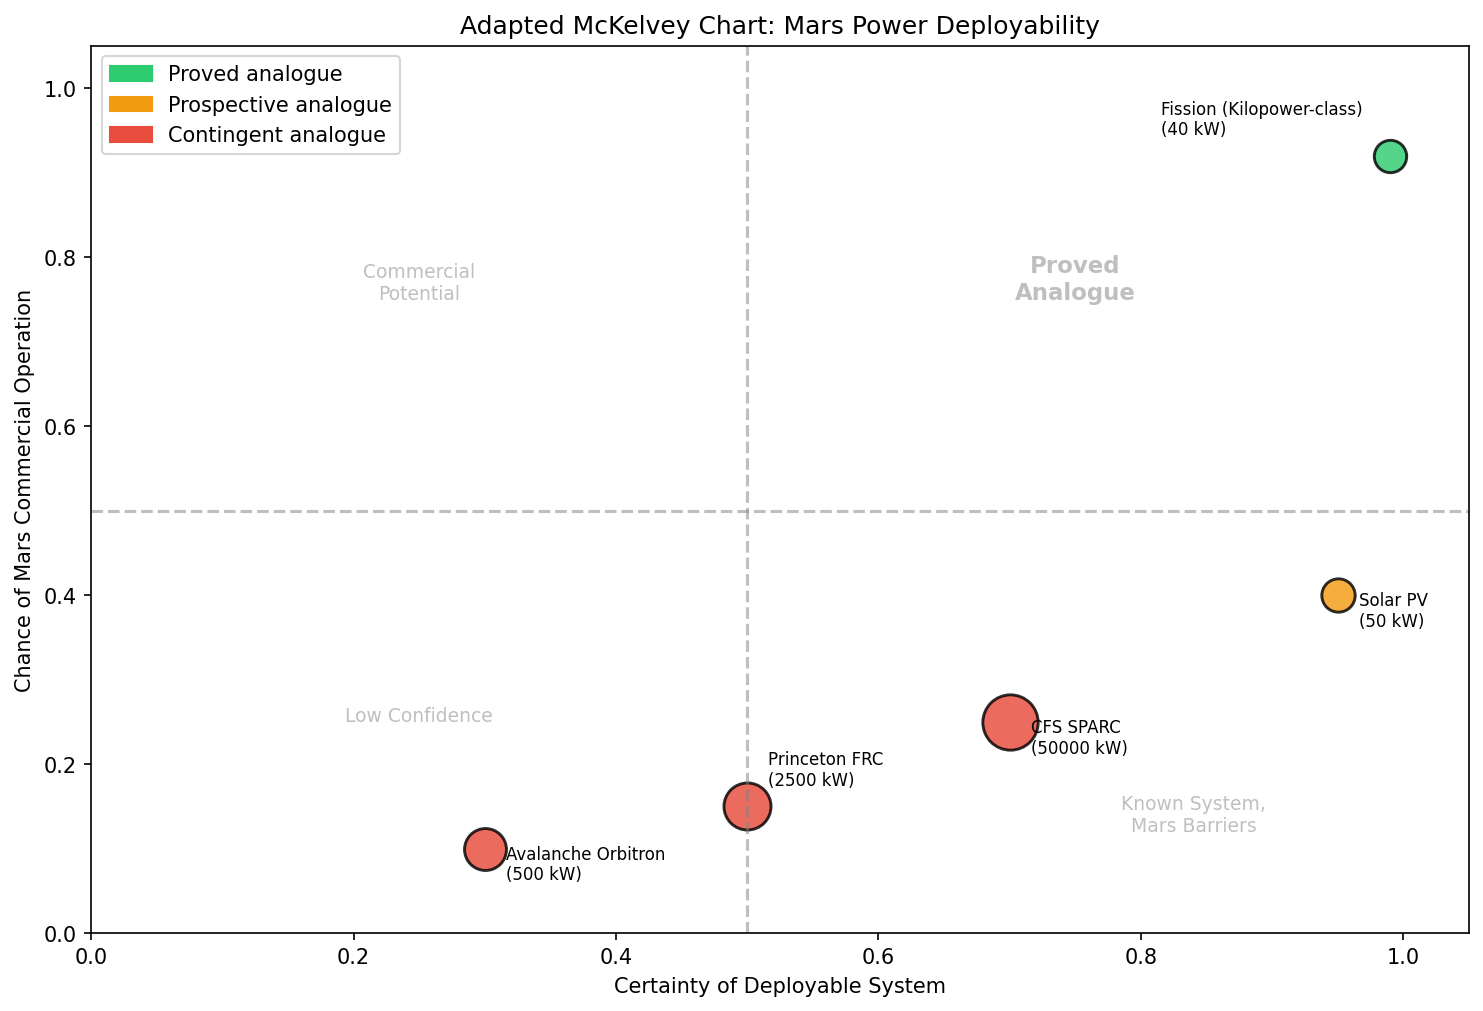
\includegraphics[width=0.82\textwidth]{mckelvey_box.png}
    \caption{McKelvey style resource classification for the five power options.}
\end{figure}

The cost model points in a different direction. On projected scale and cost, SPARC style fusion looks far cheaper than the other options. Solar and small fission units both remain expensive after launch is included.

\begin{table}[H]
    \centering
    \caption{Base LCOE results with launch cost included.}
    \label{tab:lcoe}
    \begin{tabular}{>{\raggedright\arraybackslash}p{2.7in}r}
        \toprule
        Source & LCOE (\$/kWh) \\
        \midrule
        Solar PV & 7.61 \\
        Fission, Kilopower class & 8.31 \\
        CFS SPARC & 0.64 \\
        Princeton FRC & 2.16 \\
        Avalanche Orbitron & 2.30 \\
        \bottomrule
    \end{tabular}
\end{table}

\begin{figure}[H]
    \centering
    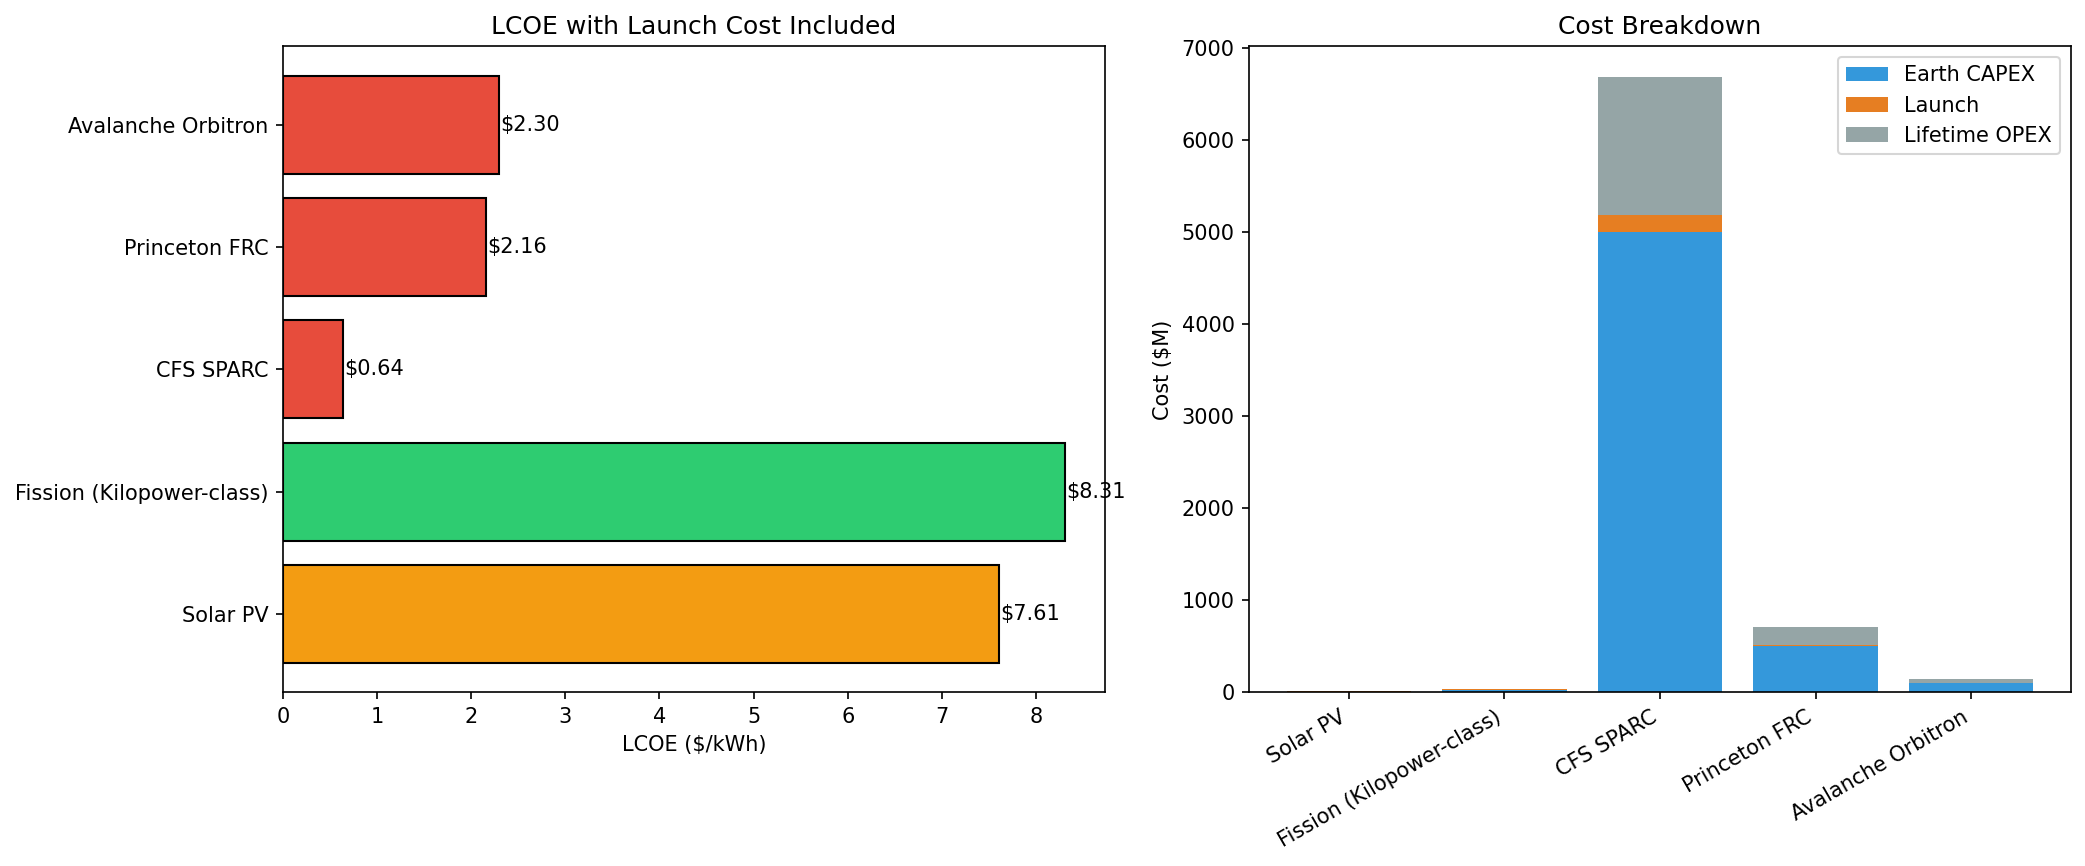
\includegraphics[width=\textwidth]{lcoe_comparison.png}
    \caption{All in cost comparison. The left panel shows LCOE and the right panel shows the cost breakdown.}
\end{figure}

Taken together, these two figures show the central tension in the project. Fission looks much more deployable now, but fusion looks stronger if the question is long run scale and projected cost.

\subsection{Reliability under dust storms}

The reliability results are much less ambiguous. The 6 person baseline case with solar plus fission is effectively perfect in the simulation, with a mean reliability of 1.0000 and a 5th percentile of 1.0000.

\begin{figure}[H]
    \centering
    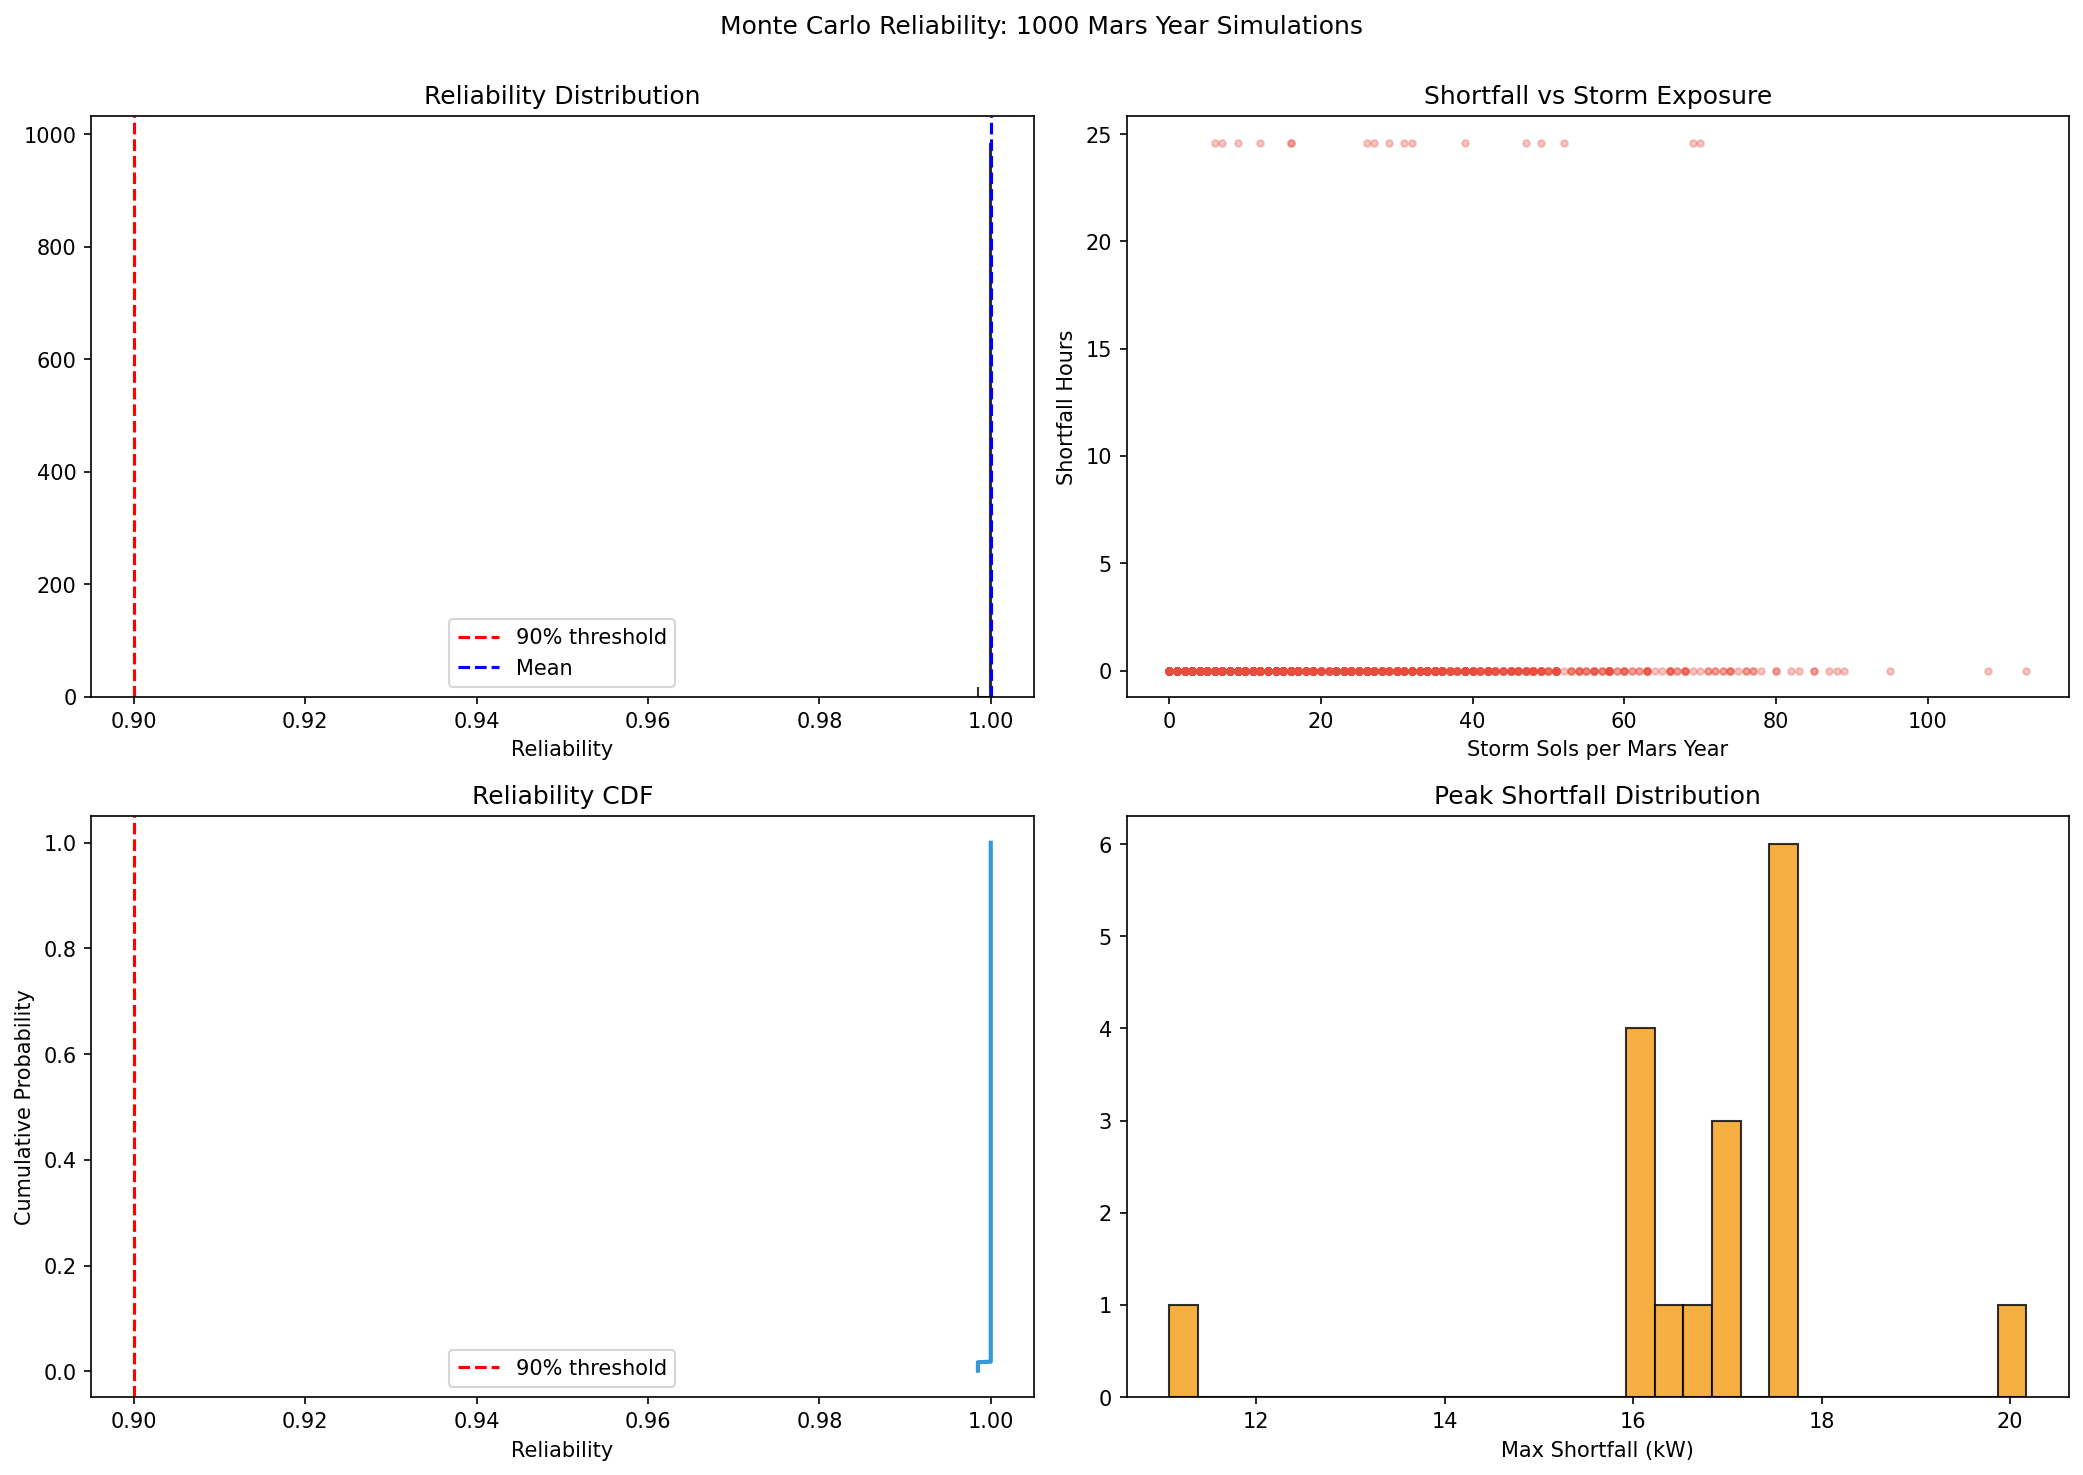
\includegraphics[width=\textwidth]{monte_carlo_reliability.png}
    \caption{Baseline Monte Carlo reliability for the 6 person solar plus fission case.}
\end{figure}

The scenario comparison is the clearest result in the report. Solar only systems perform poorly at every colony size we tested, while solar plus fission stays near full reliability.

\begin{table}[H]
    \centering
    \caption{Scenario reliability summary from the full simulation run.}
    \label{tab:scenarios}
    \begin{tabular}{>{\raggedright\arraybackslash}p{2.4in}rrr}
        \toprule
        Scenario & Mean reliability & 5th percentile & Zero shortfall share \\
        \midrule
        6p Solar only & 0.1379 & 0.1107 & 0.000 \\
        6p Solar plus Fission & 1.0000 & 1.0000 & 0.984 \\
        100p Solar only & 0.2123 & 0.1796 & 0.000 \\
        100p Solar plus Fission & 0.9960 & 0.9910 & 0.062 \\
        2000p Solar only & 0.2068 & 0.1751 & 0.000 \\
        2000p Solar plus Fission & 0.9958 & 0.9910 & 0.070 \\
        \bottomrule
    \end{tabular}
\end{table}

\begin{figure}[H]
    \centering
    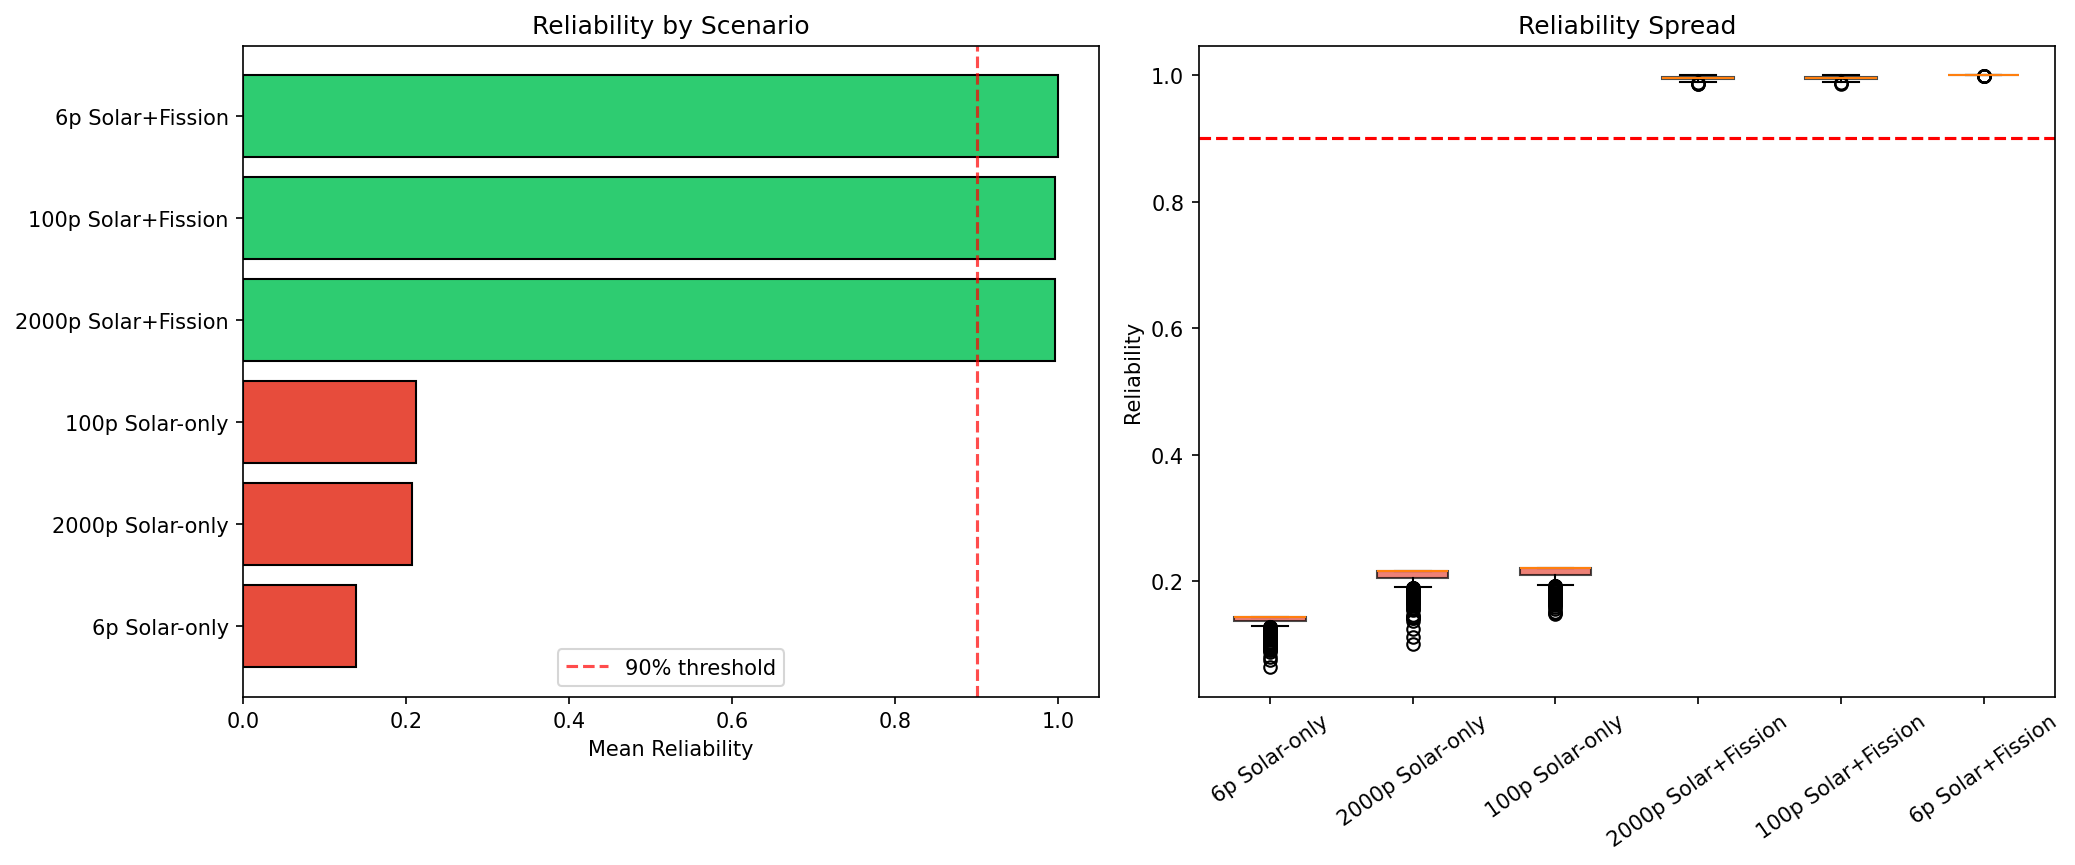
\includegraphics[width=\textwidth]{scenario_reliability.png}
    \caption{Reliability across colony size and supply mix.}
\end{figure}

\subsection{Scaling and sensitivity}

The scaling studies explain why fusion still matters in the project even though fission wins the near term reliability argument. For the 100 person colony, 8 Kilopower units are enough to cross 90 percent mean reliability. For the 2{,}000 person colony, the same threshold takes 160 units. That does not make large scale fission impossible, but it does show why the logistics become unattractive.

\begin{figure}[H]
    \centering
    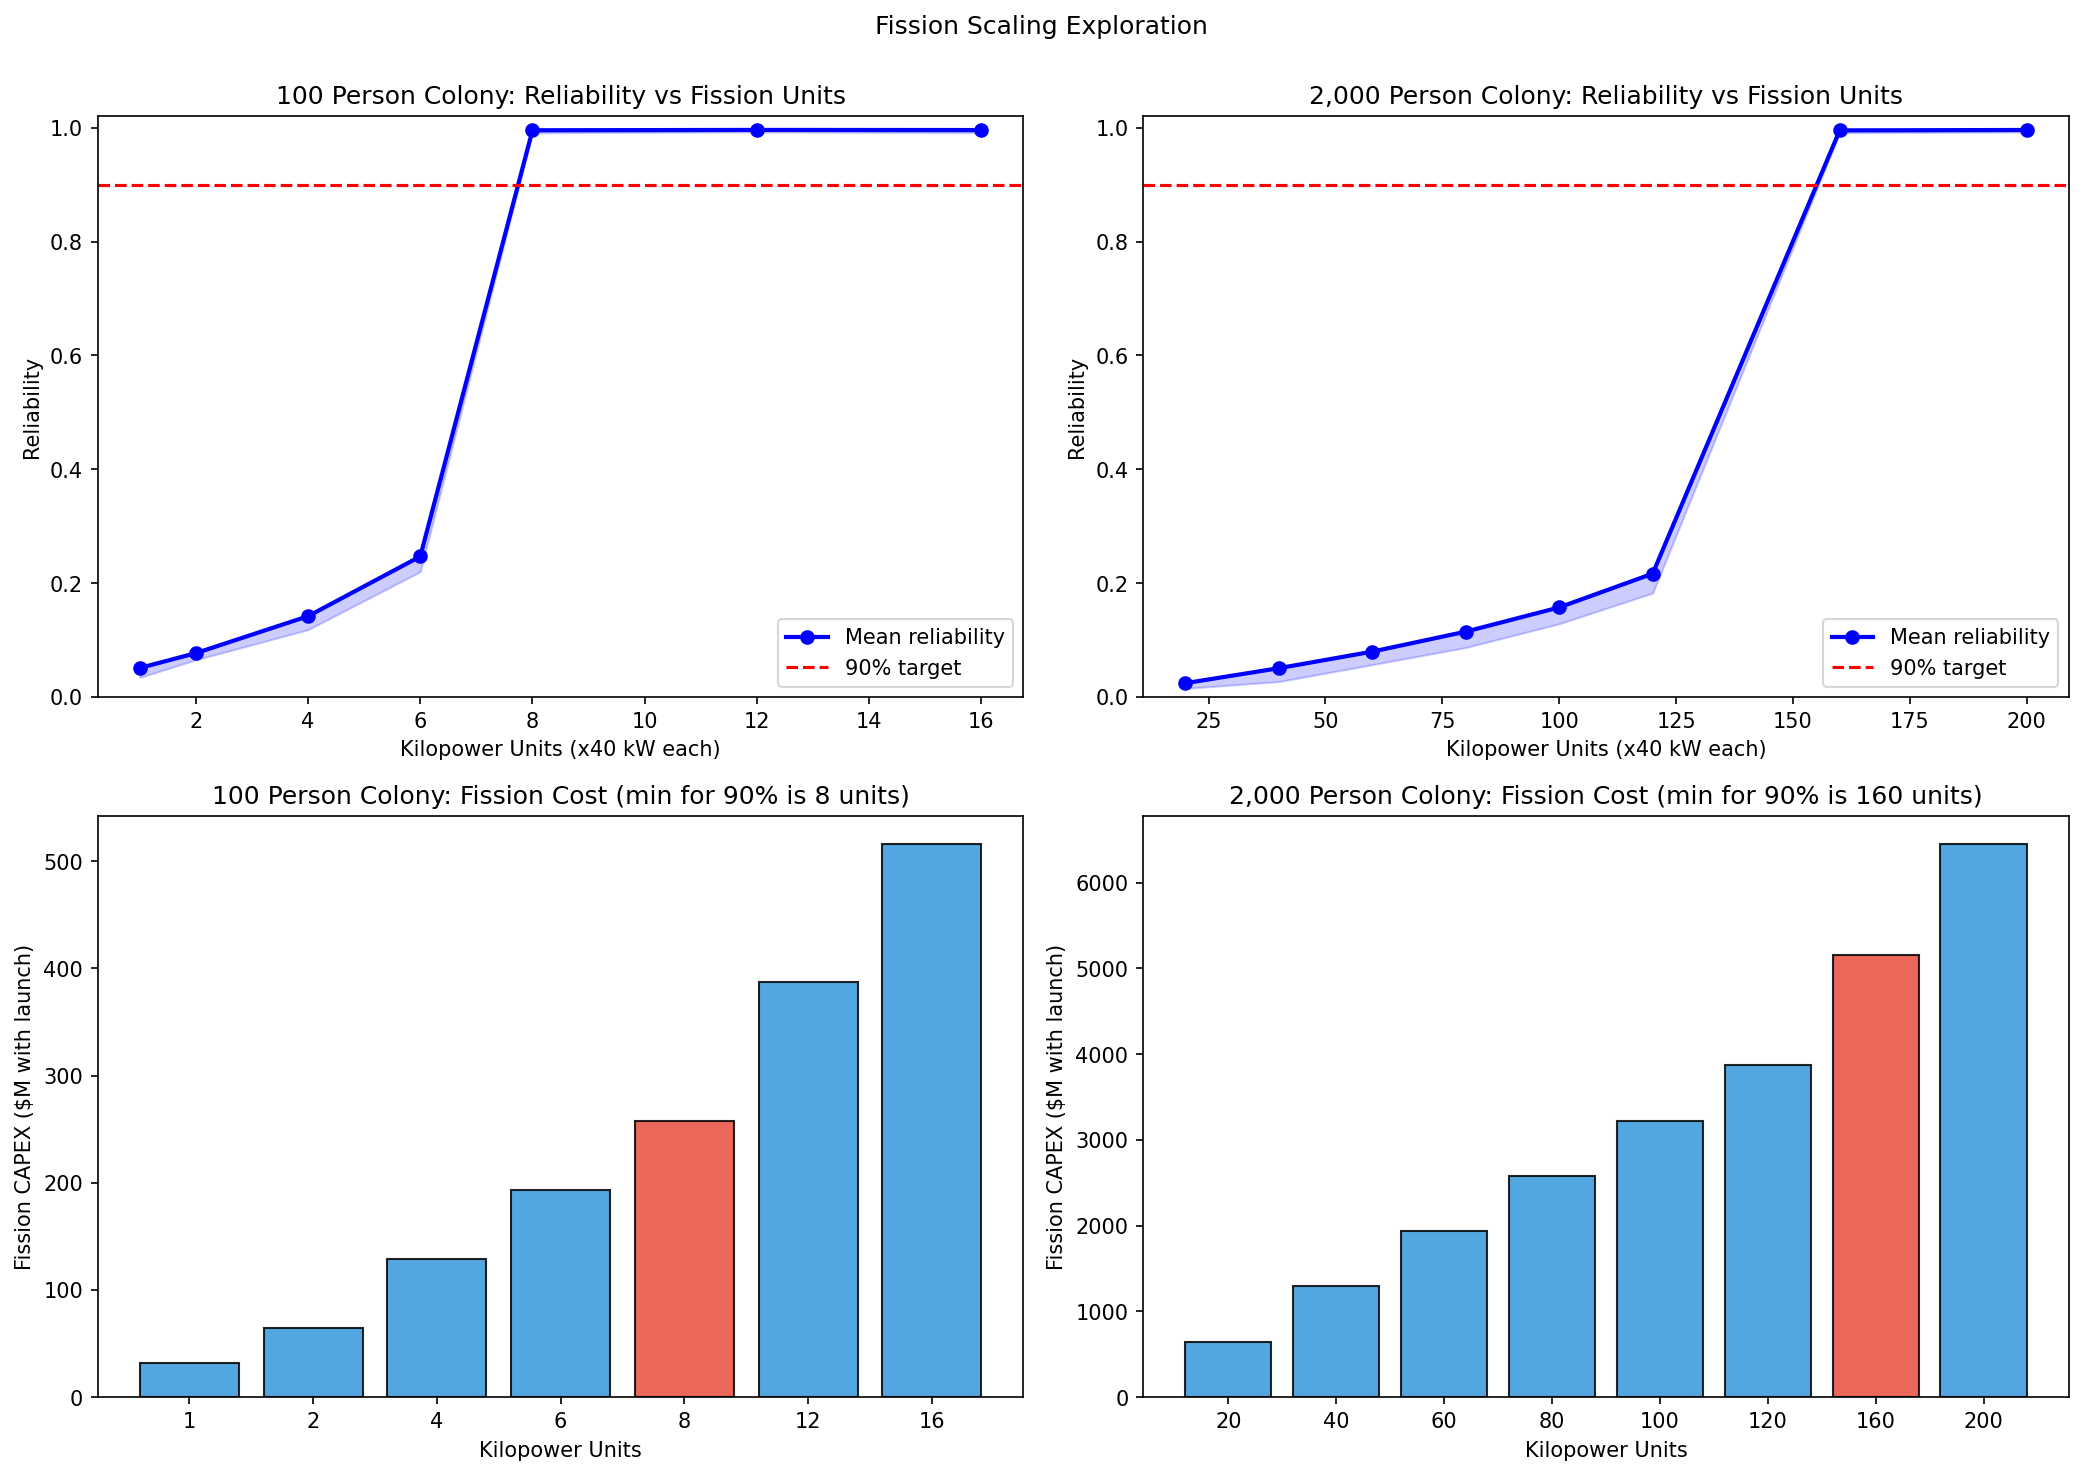
\includegraphics[width=\textwidth]{fission_scaling.png}
    \caption{Fission scaling for the 100 person and 2{,}000 person cases.}
\end{figure}

The sensitivity work does not overturn the basic story. The TRL mapping changes the exact fusion placement in the feasibility chart, and launch cost can move the ordering near the bottom of the LCOE ranking, but none of those changes make fusion mature today or make solar only systems reliable.

\begin{figure}[H]
    \centering
    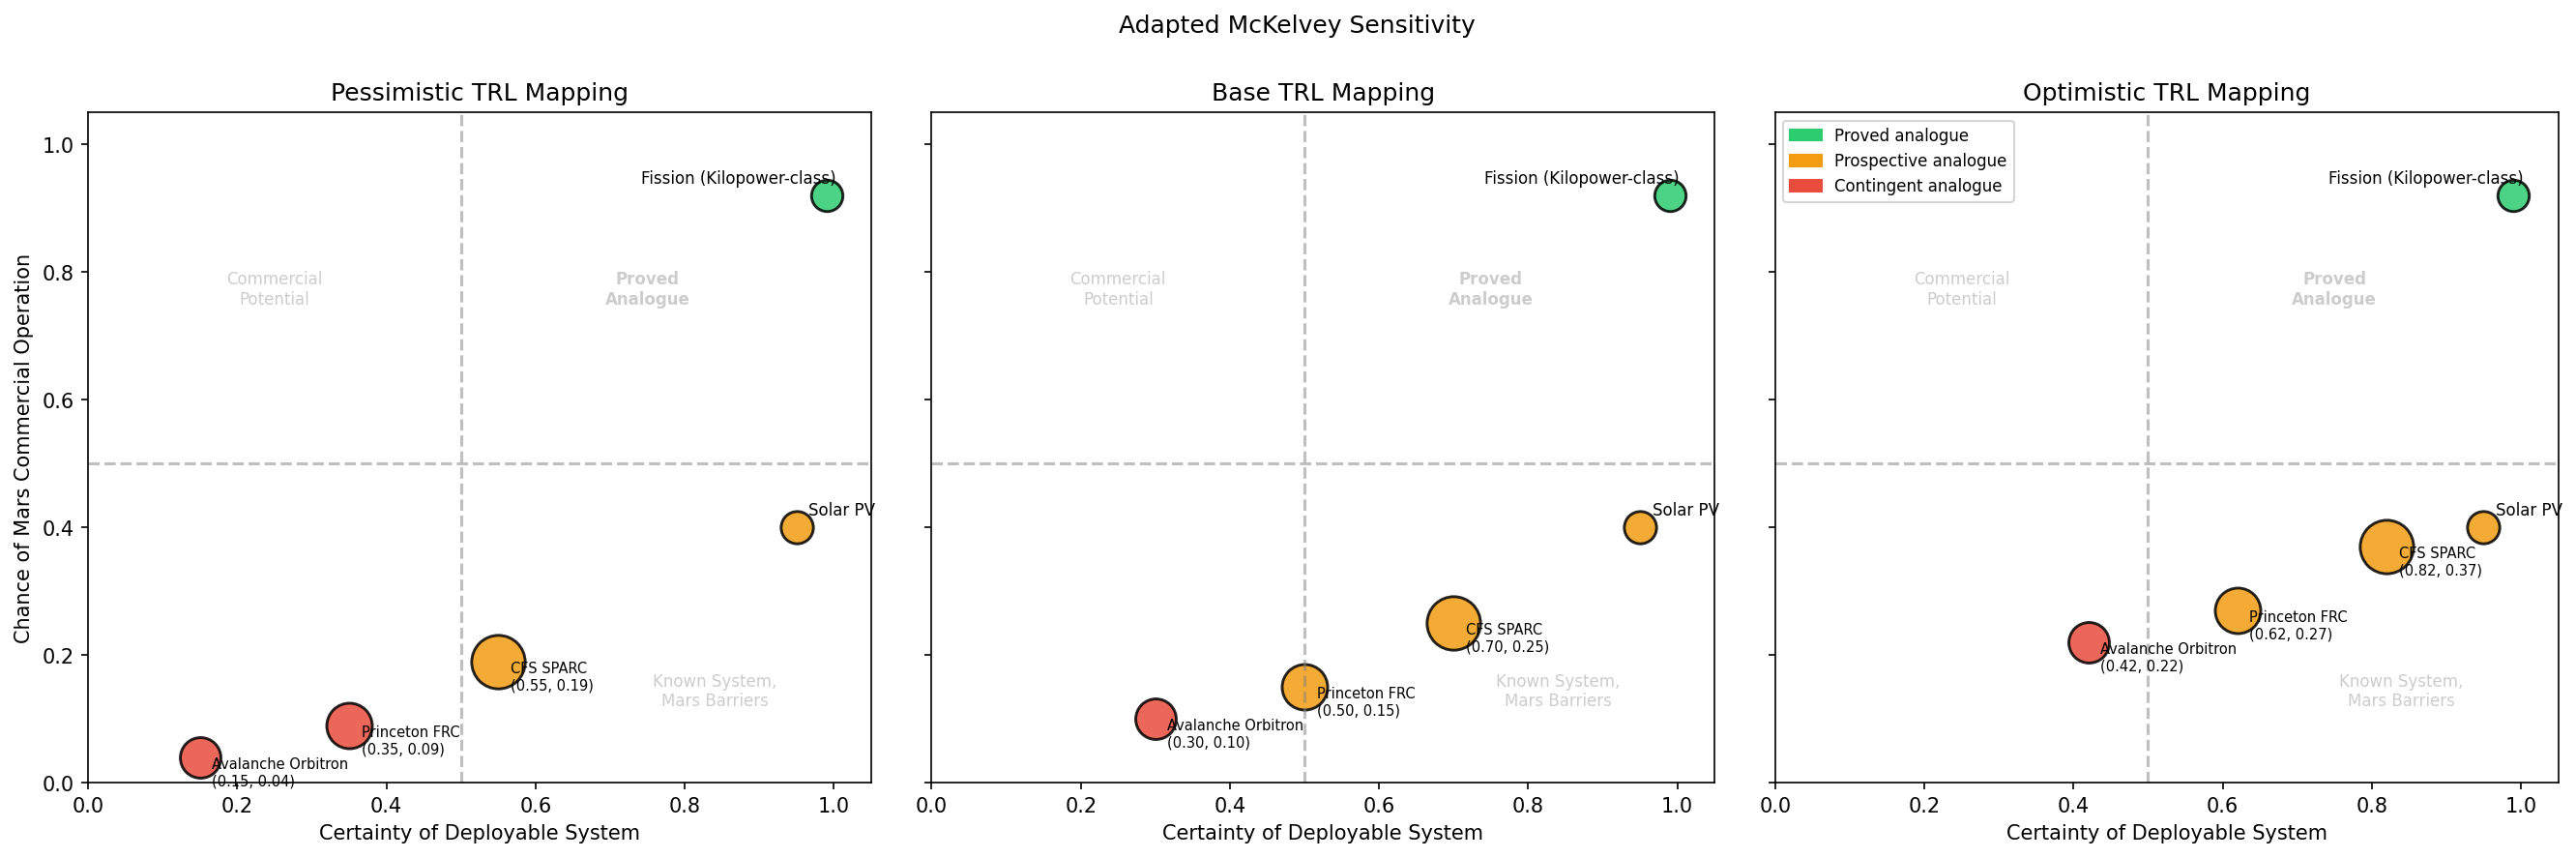
\includegraphics[width=\textwidth]{mckelvey_sensitivity.png}
    \caption{McKelvey sensitivity to different maturity assumptions.}
\end{figure}

\begin{figure}[H]
    \centering
    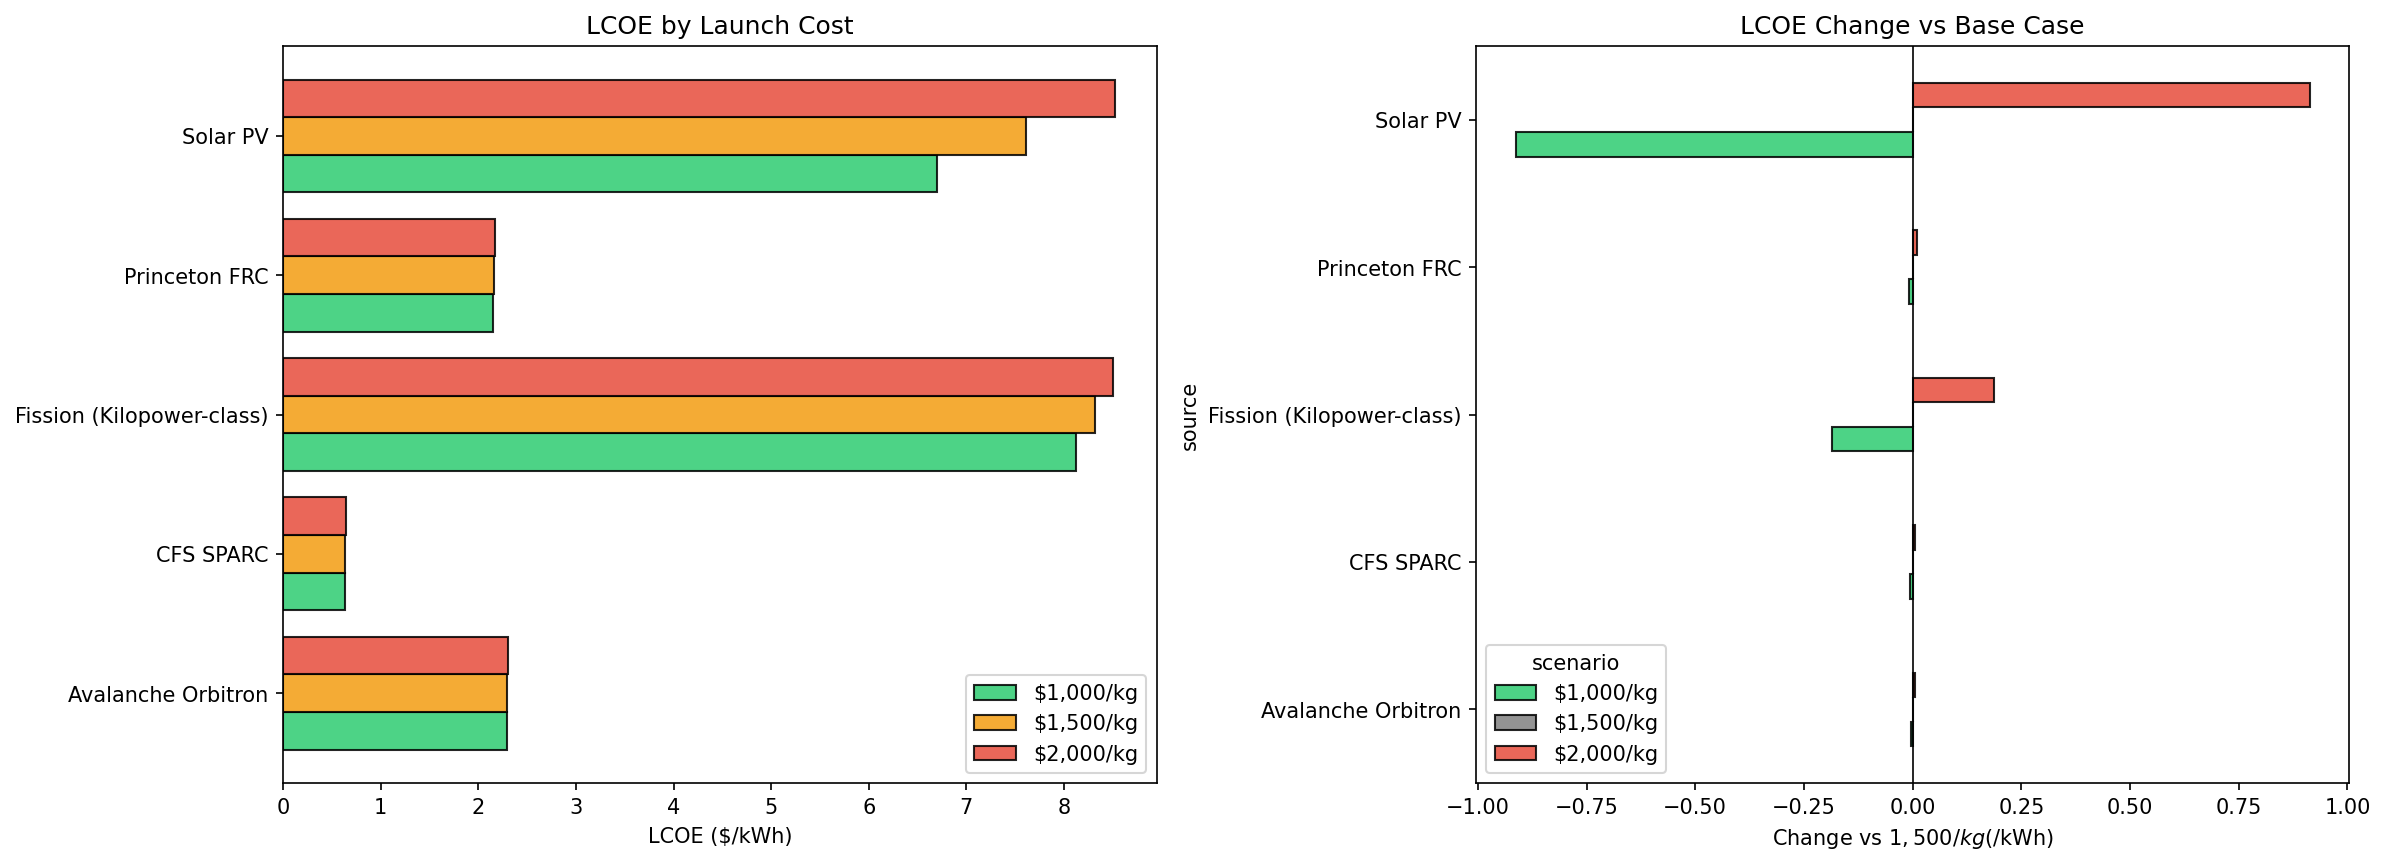
\includegraphics[width=\textwidth]{lcoe_sensitivity.png}
    \caption{LCOE sensitivity to launch cost.}
\end{figure}

\begin{figure}[H]
    \centering
    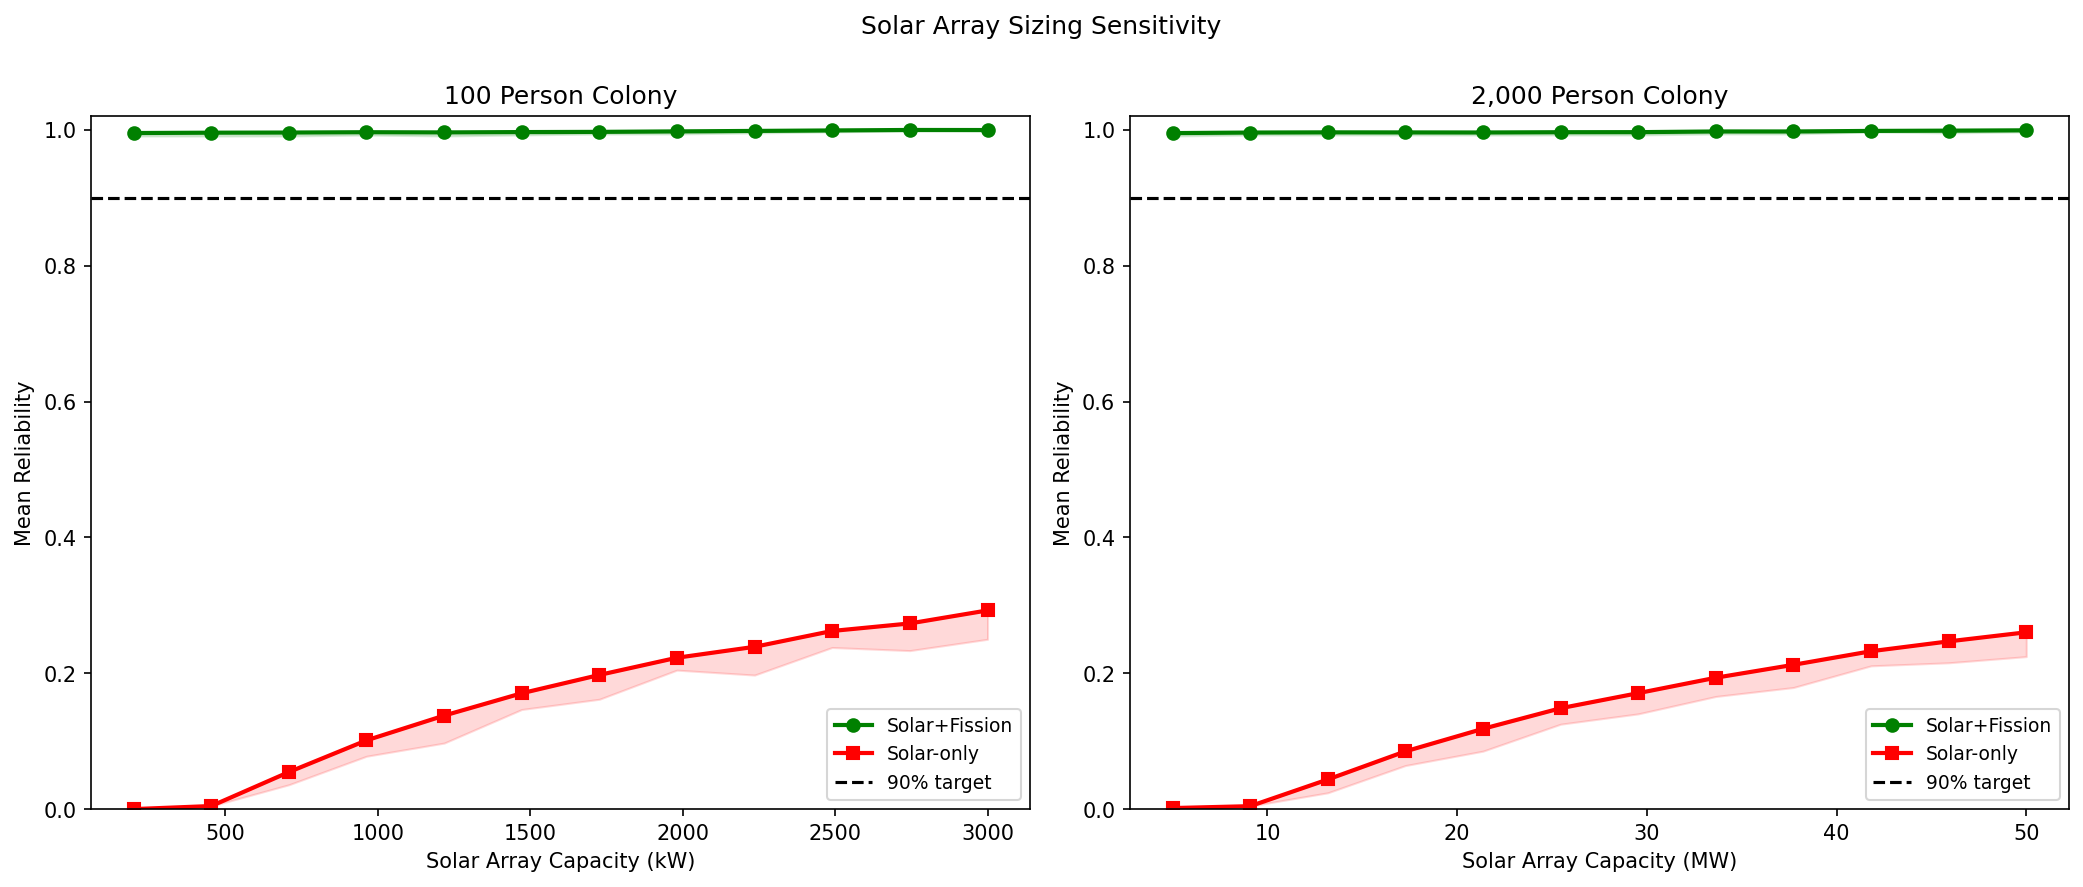
\includegraphics[width=\textwidth]{solar_sizing_sensitivity.png}
    \caption{Solar sizing sensitivity for larger colonies.}
\end{figure}

\begin{figure}[H]
    \centering
    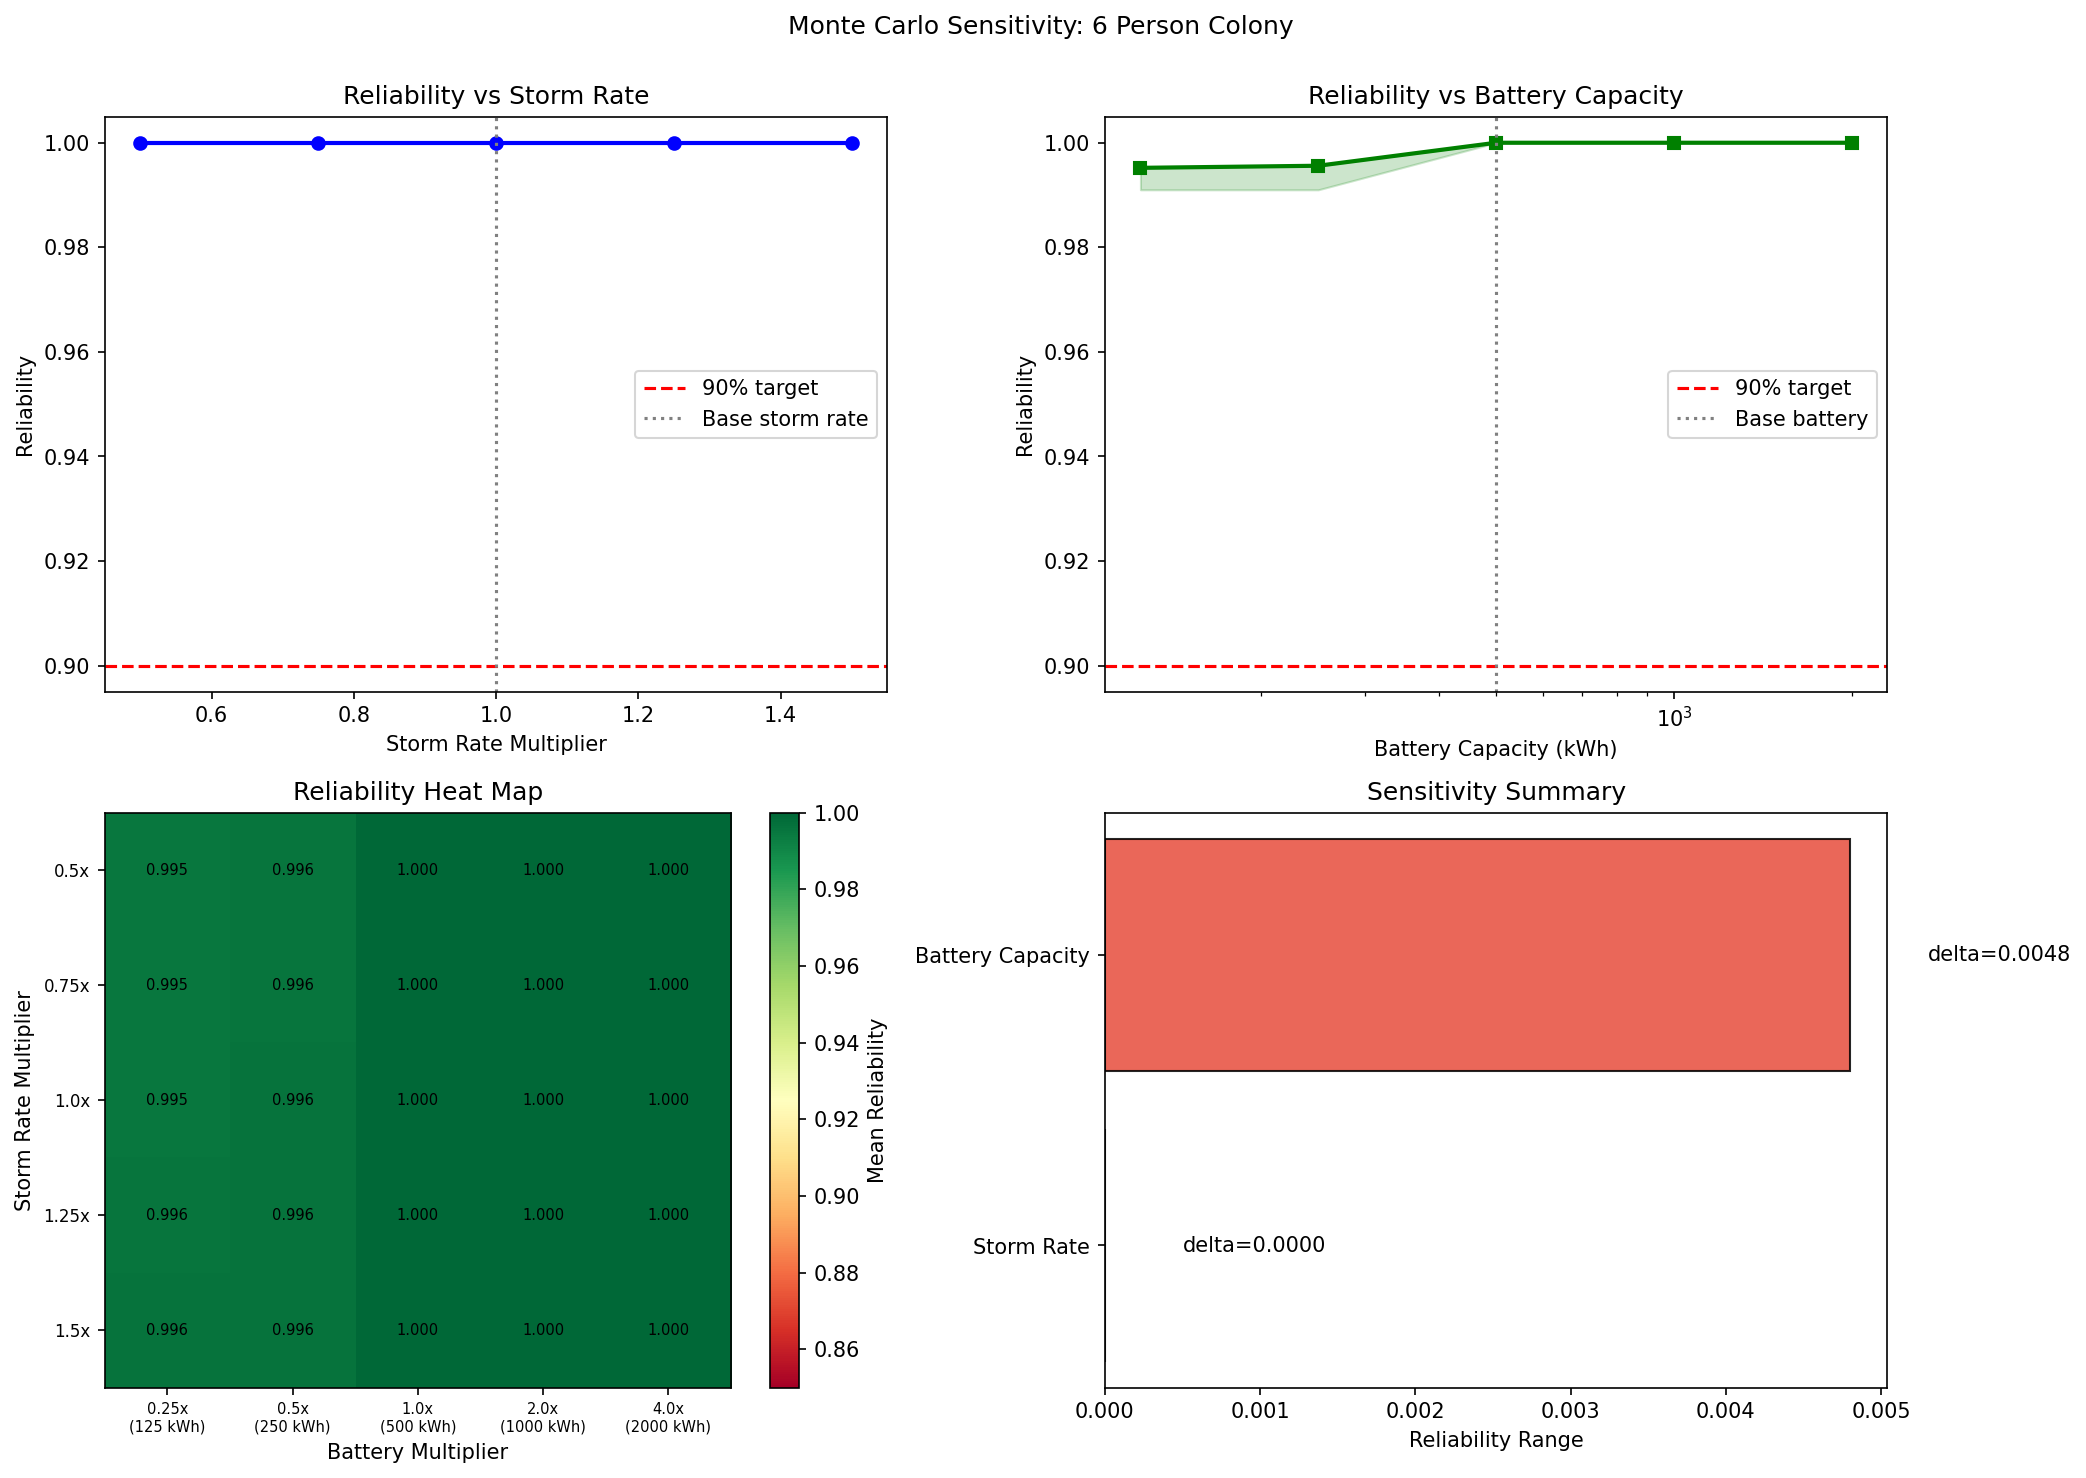
\includegraphics[width=\textwidth]{monte_carlo_sensitivity.png}
    \caption{Reliability sensitivity to storm rate and battery size in the 6 person baseline case.}
\end{figure}

\subsection{Forecast comparison}

The forecast comparison is secondary, but it is still internally consistent. The Transformer proxy gives the lowest error for all three colony sizes.

\begin{figure}[H]
    \centering
    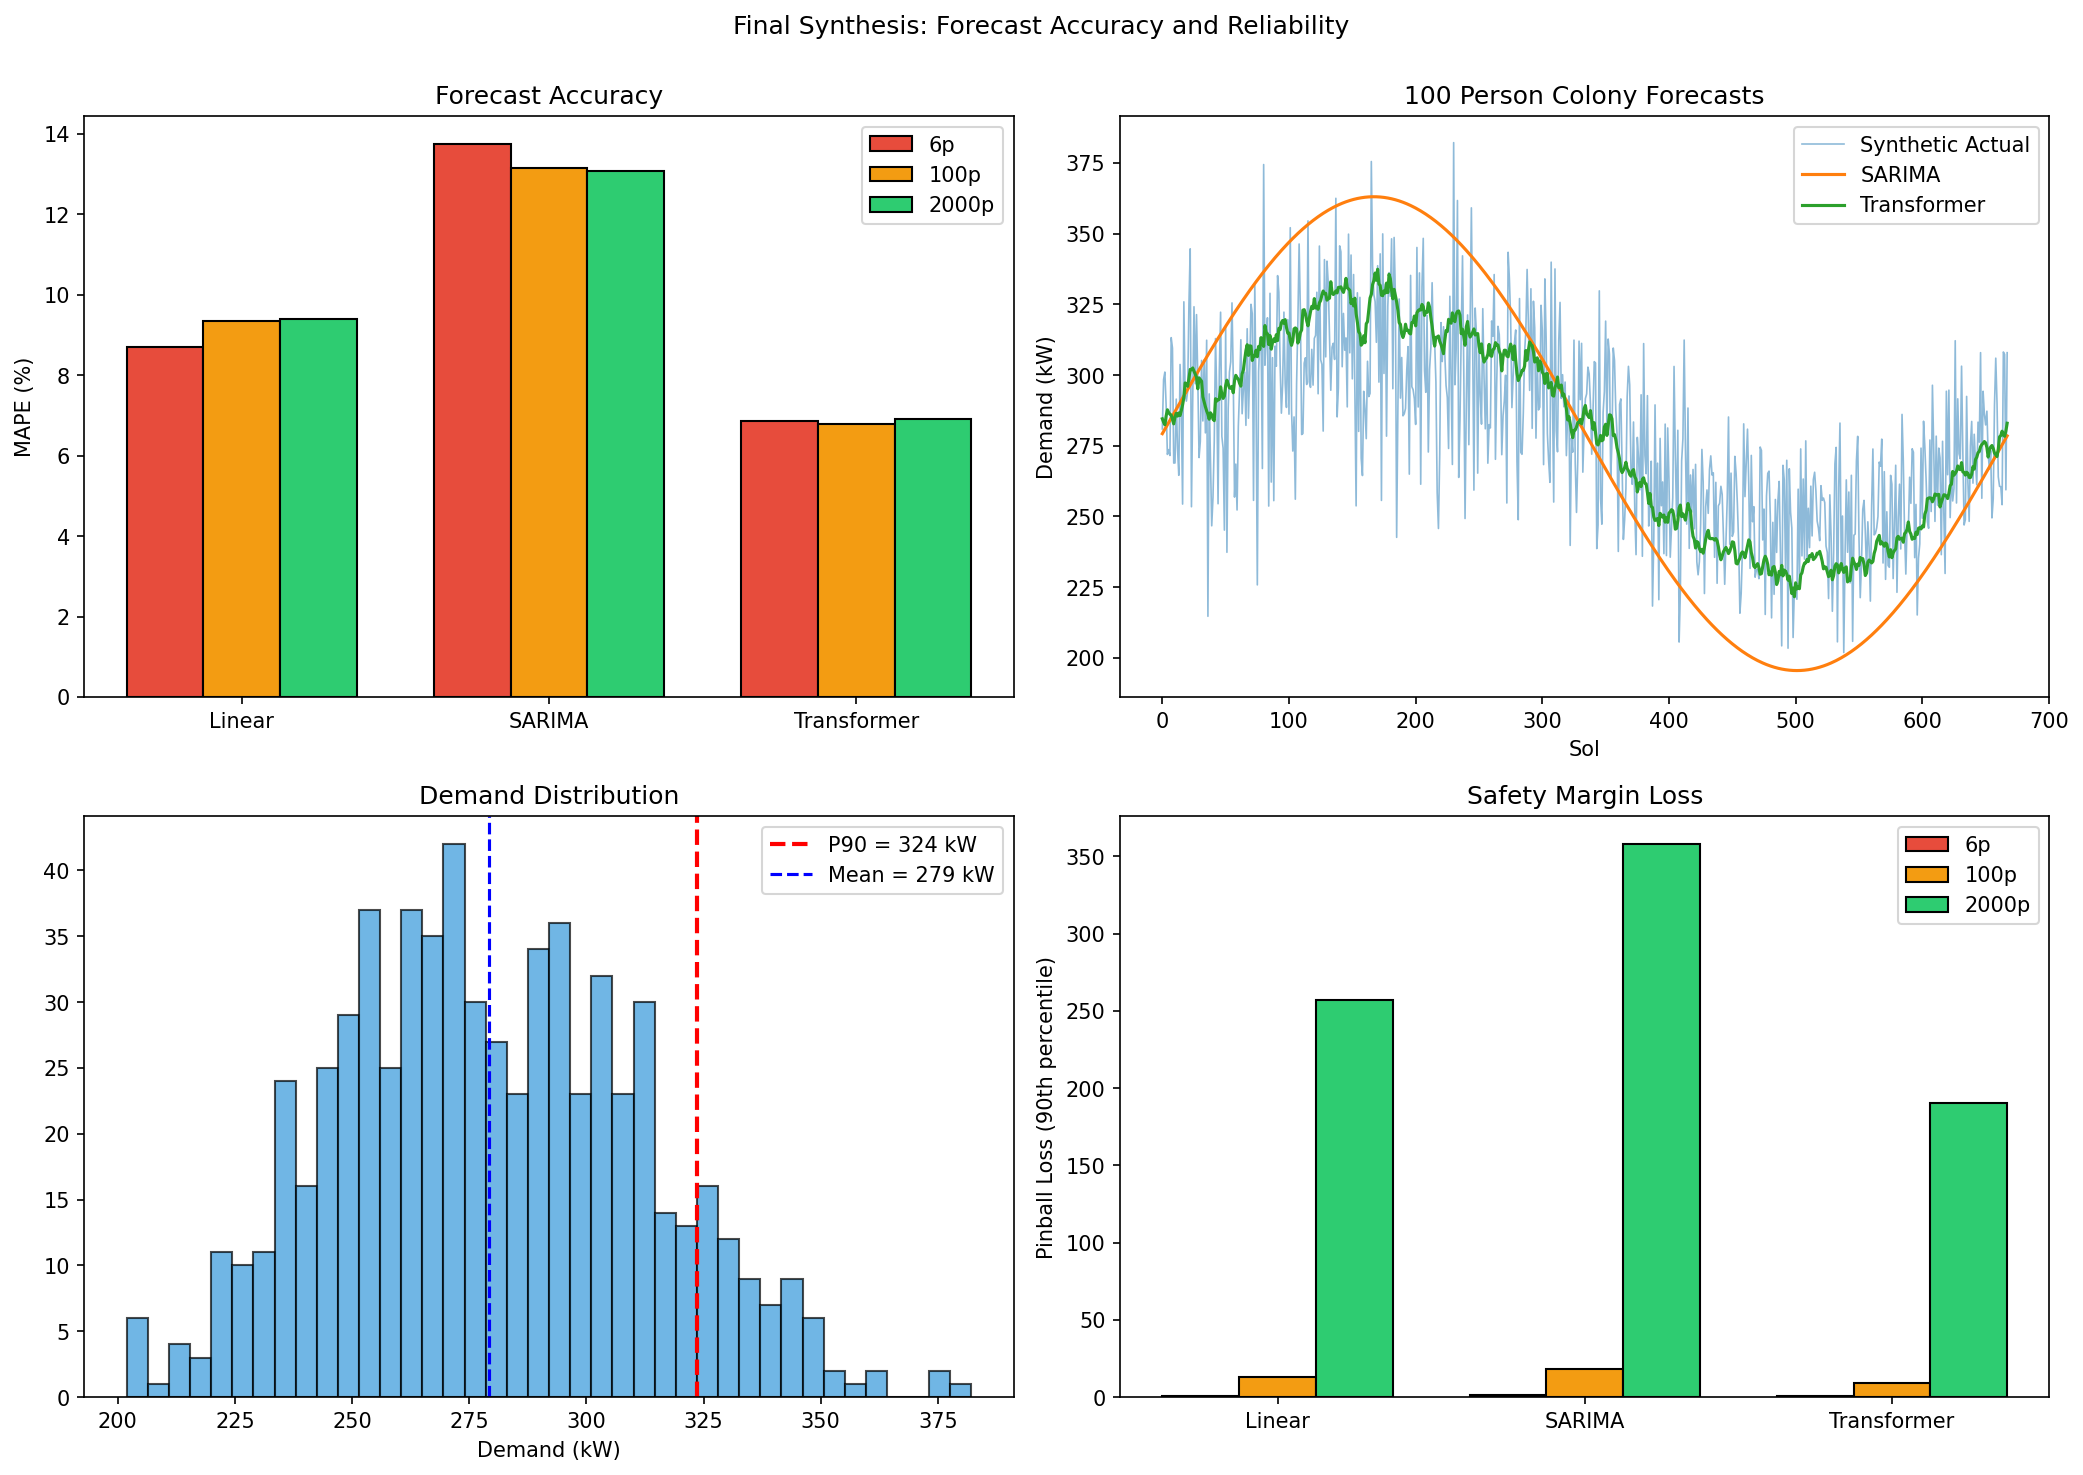
\includegraphics[width=\textwidth]{final_synthesis.png}
    \caption{Forecast comparison summary.}
\end{figure}

\section{Discussion}

The project supports a simple conclusion. If the goal is a power system that looks credible with current technology, fission with solar support is the strongest answer in this repo. If the goal is to think about very large colony scale decades in the future, fusion becomes more attractive because the cost model and the fission scaling study both point in that direction.

At the same time, the report should be clear about what is assumed rather than observed. The dust penalty curve is simplified. The habitat constants and storage tables are project inputs, not downloaded field datasets. Fusion performance numbers come from public concept descriptions, not operating reactors. Those limits do not erase the result, but they do set the right level of confidence.

\section{Reproducibility}

The project can be regenerated from the repo with:

\begin{center}
\path{.venv/bin/python run_analysis.py}
\end{center}

The input CSV source record is in:

\begin{center}
\path{docs/DATA_SOURCES.md}
\end{center}

The GitHub repository for the submitted project is:

\begin{center}
\href{https://github.com/sjheinz17/MarsColonyNuclearFusion}{https://github.com/sjheinz17/MarsColonyNuclearFusion}
\end{center}

\section{Conclusion}

This project does not argue that fusion is ready for Mars now. It argues that the case for fusion becomes stronger as colony scale grows, while the practical case for the first serious Mars power system still points to fission with solar support. That is the main result that stays stable across the classification work, the cost model, and the dust storm reliability analysis.

\begin{thebibliography}{9}

\bibitem{dra}
National Aeronautics and Space Administration.
\newblock \emph{Human Exploration of Mars Design Reference Architecture 5.0}.
\newblock NASA, 2010.

\bibitem{mdad}
J. M. Battalio and H. Wang.
\newblock \emph{The Mars Dust Activity Database}.
\newblock Icarus, 354, 2021.

\bibitem{eia}
U.S. Energy Information Administration.
\newblock \emph{Electric Power Annual, Table 4.08.B. Capacity Factors for Utility Scale Generators Primarily Using Non-Fossil Fuels}.

\bibitem{sparc}
A. J. Creely et al.
\newblock \emph{Overview of the SPARC tokamak}.
\newblock Journal of Plasma Physics, 86, 2020.

\bibitem{pss}
Princeton Satellite Systems.
\newblock \emph{Fusion Power for a Mission to Mars}.

\bibitem{avalanche}
Avalanche Energy.
\newblock \emph{Orbitron}.

\bibitem{moxie}
M. H. Hecht et al.
\newblock \emph{Mars Oxygen ISRU Experiment}.
\newblock Science Advances, 8, 2022.

\end{thebibliography}

\end{document}
